\documentclass[12pt]{article}\usepackage[]{graphicx}\usepackage[]{color}
% maxwidth is the original width if it is less than linewidth
% otherwise use linewidth (to make sure the graphics do not exceed the margin)
\makeatletter
\def\maxwidth{ %
  \ifdim\Gin@nat@width>\linewidth
    \linewidth
  \else
    \Gin@nat@width
  \fi
}
\makeatother

\definecolor{fgcolor}{rgb}{0.345, 0.345, 0.345}
\newcommand{\hlnum}[1]{\textcolor[rgb]{0.686,0.059,0.569}{#1}}%
\newcommand{\hlstr}[1]{\textcolor[rgb]{0.192,0.494,0.8}{#1}}%
\newcommand{\hlcom}[1]{\textcolor[rgb]{0.678,0.584,0.686}{\textit{#1}}}%
\newcommand{\hlopt}[1]{\textcolor[rgb]{0,0,0}{#1}}%
\newcommand{\hlstd}[1]{\textcolor[rgb]{0.345,0.345,0.345}{#1}}%
\newcommand{\hlkwa}[1]{\textcolor[rgb]{0.161,0.373,0.58}{\textbf{#1}}}%
\newcommand{\hlkwb}[1]{\textcolor[rgb]{0.69,0.353,0.396}{#1}}%
\newcommand{\hlkwc}[1]{\textcolor[rgb]{0.333,0.667,0.333}{#1}}%
\newcommand{\hlkwd}[1]{\textcolor[rgb]{0.737,0.353,0.396}{\textbf{#1}}}%
\let\hlipl\hlkwb

\usepackage{framed}
\makeatletter
\newenvironment{kframe}{%
 \def\at@end@of@kframe{}%
 \ifinner\ifhmode%
  \def\at@end@of@kframe{\end{minipage}}%
  \begin{minipage}{\columnwidth}%
 \fi\fi%
 \def\FrameCommand##1{\hskip\@totalleftmargin \hskip-\fboxsep
 \colorbox{shadecolor}{##1}\hskip-\fboxsep
     % There is no \\@totalrightmargin, so:
     \hskip-\linewidth \hskip-\@totalleftmargin \hskip\columnwidth}%
 \MakeFramed {\advance\hsize-\width
   \@totalleftmargin\z@ \linewidth\hsize
   \@setminipage}}%
 {\par\unskip\endMakeFramed%
 \at@end@of@kframe}
\makeatother

\definecolor{shadecolor}{rgb}{.97, .97, .97}
\definecolor{messagecolor}{rgb}{0, 0, 0}
\definecolor{warningcolor}{rgb}{1, 0, 1}
\definecolor{errorcolor}{rgb}{1, 0, 0}
\newenvironment{knitrout}{}{} % an empty environment to be redefined in TeX

\usepackage{alltt}

%\usepackage[roman]{../pres1}
%\usepackage[sans]{../pres1}

\usepackage[hmargin=1in,vmargin=1in]{geometry}
\usepackage{parskip}
\usepackage{hyperref}
\usepackage{graphicx}
\hypersetup{pdfstartview=FitV,hidelinks}



\IfFileExists{upquote.sty}{\usepackage{upquote}}{}
\begin{document}

{
  \Large
  \centering
  Lab 5 Assignment --- Models of Interspecific Interactions \\
  Due by Monday \par
}

Answer each of the following questions and upload your Excel file (and
R script) to ELC. Be sure to show your calculations. Name the 
file something like: \texttt{Chandler\_Richard\_lab4.xlsx}. \\



\vspace{6pt}

{\bf Exercise I \\}
You are studying the dynamics of jaguar (\textit{Panthera onca}) and Baird's
tapir (\textit{Tapirus bairdii}) in Costa Rica's Corcavodo National Park. After
years of research, you obtain the following parameter estimates, which
you would like to use in a Lotka-Volterra model: $r^{prey}=0.05$,
$d^{prey}=0.0005$, $b^{pred}=0.001$, and $d^{pred}=0.45$.  
\begin{enumerate}
  \item[(a)] What predator population size corresponds to prey equilibrium?
    What prey population size corresponds to predator equilibrium? 
  \item[(b)] Project the populations 50 years following an initial prey
    population size of $N_0^{prey}=500$ and an initial predator
    population size of $N_0^{pred}=100$. Plot the projections.  
  \item[(c)] Clearly, these populations have not reached a stable
    equilibrium, so what is the interpretation of the equilibrium
    values from part (a)? What happens if you set the initial
    population sizes to the equilibrium values?  
  \item[(d)] Change the value of $r^{prey}$ from 0.05 to 0.1,
    and recalculate the equilibrium points for prey and
    predators. Project the dynamics of both species again. Plot the
    results. What are the primary differences?  What explains these
    differences? 
\end{enumerate}

\vspace{12pt}

\begin{figure}[h!]
  \centering
  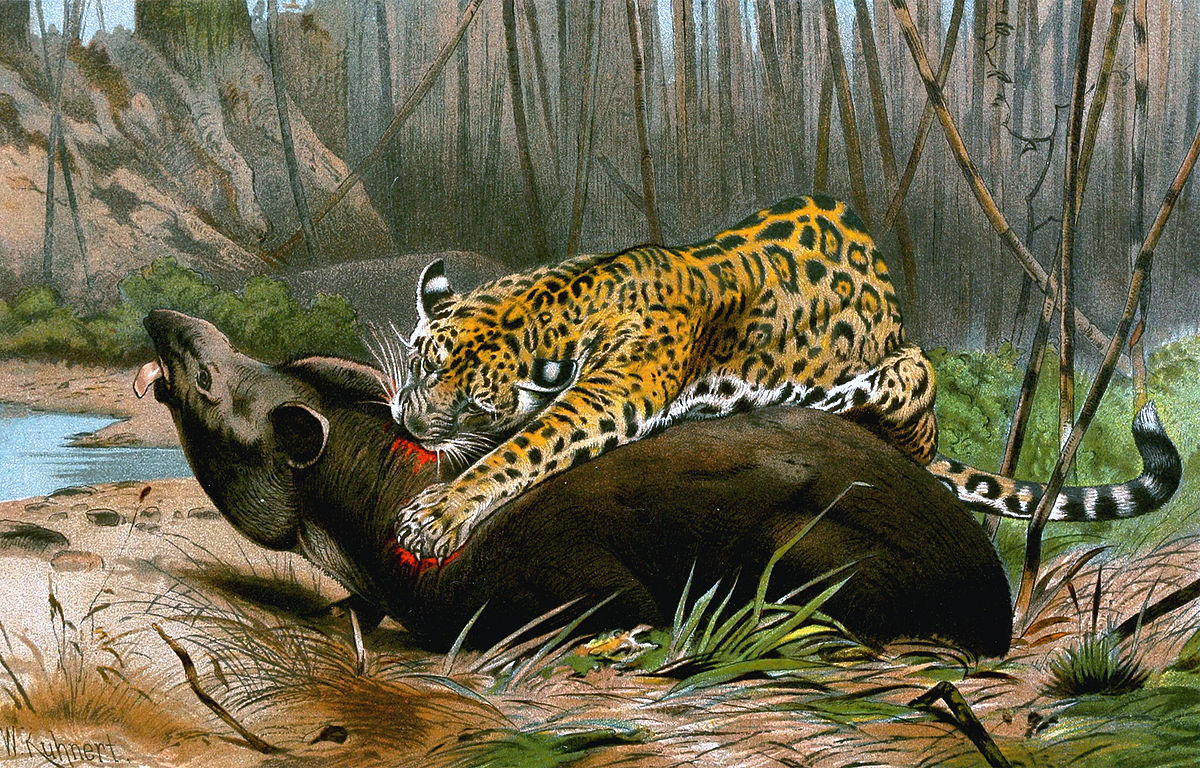
\includegraphics[width=0.85\textwidth]{jaguar_killing_tapir}
%  \caption{Jaguar and tapir}
  \label{fig:jag-tapir}
\end{figure}


\clearpage

{\bf Exercise II \\}
The Canada warbler (\textit{Cardellina canadensis}) and the hooded
warbler ({\it Stetophaga citrina}) are two species of
Neotropical-Nearctic migratory birds that appear to compete for the
same resources where their ranges meet in the southern Appalachian
Mountains. Assume their dynamics follow the Lotka-Volterra competition
model with parameters $r^{A}=0.2$, $r^{B}=0.3$,
$K^{A}=250$, $K^{B}=200$, $\alpha^{A}=0.1$, and 
$\alpha^{B}=0.1$.   
\begin{enumerate}
  \item[(a)] Plot 25 years of dynamics following initial conditions of 
    $N_0^A = 200$ and $N_0^B=50$. Do these conditions describe stable
    coexistence, competitive exclusion, or unstable equilibrium? 
  \item[(b)] What are the 2 equilibrium values for these species?
  \item[(c)] What is the minimum value of $\alpha^B$ that would result in
    competitive exclusion of species A? (Hint: Use the equilibrium
    equations to solve for $\alpha^B$). Plot 25 years of dynamics under
    this scenario. Use the same initial abundance values as before. 
\end{enumerate}


\vspace{12pt}

\begin{figure}[h!]
  \centering
  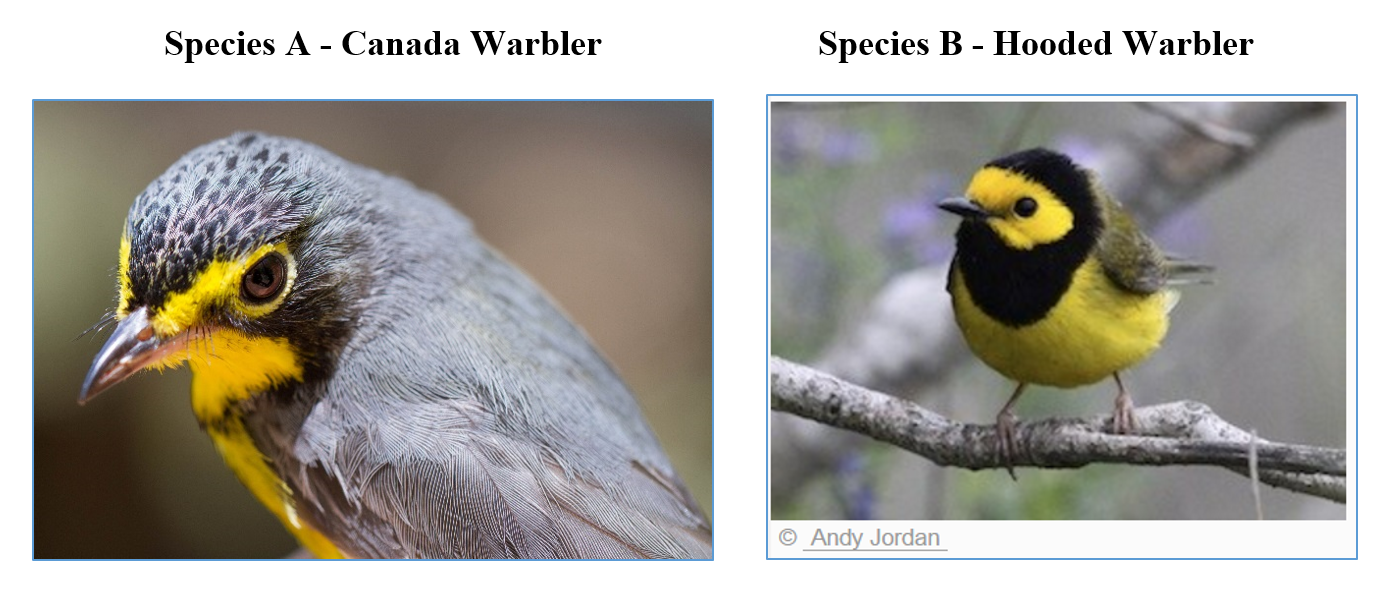
\includegraphics[width=\textwidth]{cawa-howa}
  \label{fig:cawa-howa}
\end{figure}


\clearpage

{\bf R example \\}


\begin{knitrout}
\definecolor{shadecolor}{rgb}{0.969, 0.969, 0.969}\color{fgcolor}\begin{kframe}
\begin{alltt}
\hlstd{nYears} \hlkwb{<-} \hlnum{5000}
\hlstd{r.prey} \hlkwb{<-} \hlnum{0.01}
\hlstd{d.prey} \hlkwb{<-} \hlnum{0.00001}
\hlstd{b.pred} \hlkwb{<-} \hlnum{0.00001}
\hlstd{d.pred} \hlkwb{<-} \hlnum{0.01}
\hlstd{N.prey} \hlkwb{<-} \hlkwd{rep}\hlstd{(}\hlnum{NA}\hlstd{, nYears)}
\hlstd{N.pred} \hlkwb{<-} \hlkwd{rep}\hlstd{(}\hlnum{NA}\hlstd{, nYears)}
\hlstd{N.prey[}\hlnum{1}\hlstd{]} \hlkwb{<-} \hlnum{1000}
\hlstd{N.pred[}\hlnum{1}\hlstd{]} \hlkwb{<-} \hlnum{300}
\hlkwa{for}\hlstd{(t} \hlkwa{in} \hlnum{2}\hlopt{:}\hlstd{nYears) \{}
    \hlstd{N.prey[t]} \hlkwb{<-} \hlstd{N.prey[t}\hlopt{-}\hlnum{1}\hlstd{]} \hlopt{+} \hlstd{N.prey[t}\hlopt{-}\hlnum{1}\hlstd{]}\hlopt{*}\hlstd{(r.prey}\hlopt{-}\hlstd{d.prey}\hlopt{*}\hlstd{N.pred[t}\hlopt{-}\hlnum{1}\hlstd{])}
    \hlstd{N.pred[t]} \hlkwb{<-} \hlstd{N.pred[t}\hlopt{-}\hlnum{1}\hlstd{]} \hlopt{+} \hlstd{N.pred[t}\hlopt{-}\hlnum{1}\hlstd{]}\hlopt{*}\hlstd{(b.pred}\hlopt{*}\hlstd{N.prey[t}\hlopt{-}\hlnum{1}\hlstd{]} \hlopt{-} \hlstd{d.pred)}
\hlstd{\}}
\hlkwd{plot}\hlstd{(}\hlnum{1}\hlopt{:}\hlstd{nYears, N.prey,} \hlkwc{type}\hlstd{=}\hlstr{"l"}\hlstd{,} \hlkwc{col}\hlstd{=}\hlstr{"black"}\hlstd{,} \hlkwc{ylim}\hlstd{=}\hlkwd{c}\hlstd{(}\hlnum{0}\hlstd{,} \hlnum{3500}\hlstd{),}
     \hlkwc{xlab}\hlstd{=}\hlstr{"Year"}\hlstd{,} \hlkwc{ylab}\hlstd{=}\hlstr{"Abundance"}\hlstd{)}
\hlkwd{lines}\hlstd{(}\hlnum{1}\hlopt{:}\hlstd{nYears, N.pred,} \hlkwc{type}\hlstd{=}\hlstr{"l"}\hlstd{,} \hlkwc{col}\hlstd{=}\hlstr{"blue"}\hlstd{)}
\hlkwd{legend}\hlstd{(}\hlnum{1}\hlstd{,} \hlnum{3500}\hlstd{,} \hlkwd{c}\hlstd{(}\hlstr{"Prey"}\hlstd{,} \hlstr{"Predator"}\hlstd{),} \hlkwc{lty}\hlstd{=}\hlnum{1}\hlstd{,} \hlkwc{col}\hlstd{=}\hlkwd{c}\hlstd{(}\hlstr{"black"}\hlstd{,} \hlstr{"blue"}\hlstd{))}
\end{alltt}
\end{kframe}

{\centering \includegraphics[width=0.75\textwidth]{figure/pred-prey-1} 

}



\end{knitrout}



\end{document}

